\lvli{Introduction}
The aim of the experiment is to determine locally the strain applied to an optical fiber through the measure of the spectral shift. More specifically, an Optical Frequency Domain Reflectometer (OFDR), which includes a swept-frequency laser, is employed to measure the spectral shift of the distributed Rayleigh's backscattering generated along the fiber under strain.

The refraction index of a fiber is not homogeneous, hence a signal transmitted is scattered. A small part of the signal is backscattered elastically (i.e., it preserves the same frequency of the incident signal) in a process named Rayleigh's backscattering. The scattering centers are localized in well-defined positions since they are originated in the production phase of the fiber. For this reason, a characteristic feature of the Rayleigh's backscattered signal is that it is constant and unique for each fiber under equal conditions of input signal.
The backscattered spectrum depends on the local properties of the fiber in the physical point where the scattering is generated, consequently it is possible to map a physical property of interest (applied strain in our case) in a distributed manner, that is along the entire length of the fiber.
When the fiber is mechanically under strain the scattering centers change their relative position and hence the characteristic fingerprint changes (a mechanical tension causes a frequency variation in the signal). The backscattered signal results shifted in frequency, and the resulting strain can be calculated as: $$\delta f = K_{\epsilon}\delta \epsilon$$ where $\delta f$ is the spectral shift, $\delta\epsilon$ the resulting strain, and the strain constant $ K_{\epsilon} = -0.15 $. Temperature is assumed almost constant during the experiment and consequently negligible.

\lvlii{Experimental setup}
The experimental setup consists of an OFDR and a fiber sensor made coupling mechanically the fiber with the table where the weights are applied. The fibre forms a coil, as outlined in Fig. \ref{fig:setup}: in this way the external points of the fiber are most affected by the weight applied than the internal points. The fiber coil is also under the board: when the upper coil is compressed, the coil under the board is stretched, and viceversa.
\begin{figure}[H]
	\centering
	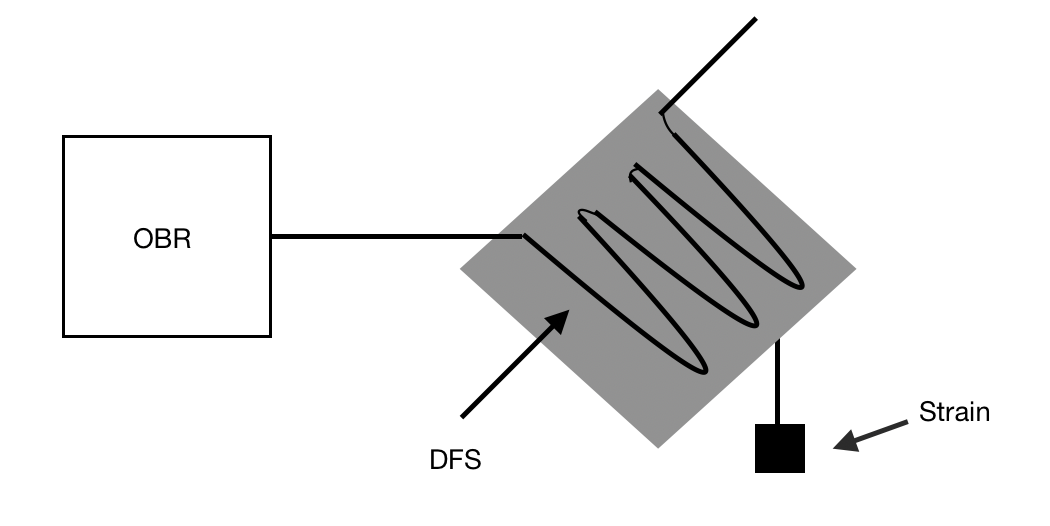
\includegraphics[height=10.5cm, width=10.5cm, keepaspectratio]{img/setup.png}
	\caption{A commercial OFDR (OBR) measures the backscattering signal of the Distributed Fiber Sensor (DFS)}\label{fig:setup}
\end{figure}
The measurements are taken increasing the weight applied as resumed in Tab.\ref{table:measures}. The measurements are taken also in the opposite direction, i.e. the weights have been removed.
\begin{table}[H]
  \centering
  \begin{tabular}{c|c|c|c}
      measure number & weight [g] & ymax [$\mu \epsilon$] & ymin [$\mu \epsilon$]\\
			\hline
      1 & 0 &  &  \\
      2 & 60 &  &  \\
      3 & 120 &  &  \\
      4 & 180 & 84.9 & -72 \\
      5 & 240 & 112 & -95 \\
      6 & 300 & 138 & -118 \\
      7 & 359 & 165 & -138 \\
      8 & 418 & 189 & -164 \\
      9 & 476 & 213 & -182 \\
      10 & 534 & 238 & -202 \\
      11 & 591 & 261 & -220 \\
      12 & 686 & 300 & -256 \\
      13 & 782 & 339 & -289 \\
      14 & 686 &  &  \\
      15 & 591 &  &  \\
      16 & 534 &  &  \\
      17 & 476 &  &  \\
      18 & 418 &  &  \\
      19 & 359 &  &  \\
      20 & 300 &  &  \\
      21 & 240 &  &  \\
      22 & 180 &  &  \\
      23 & 120 &  &  \\
      24 & 60 &  &  \\
      25 & 0 &  &  \\
  \end{tabular}
  \caption{Measurements performed.}
  \label{table:measures}
\end{table}
Electrical sensors are used to check whether the measurements conditions are positive, for example that the board is not moving.



\lvli{Analysis}
The row data collected consist in the complex envelope (amplitude and phase) of the electric field as a function of the position along two orthogonal polarization: polarization S and polarization P, as can be seen in Fig.\ref{fig:raw}.
\begin{figure}[H]
	\centering
	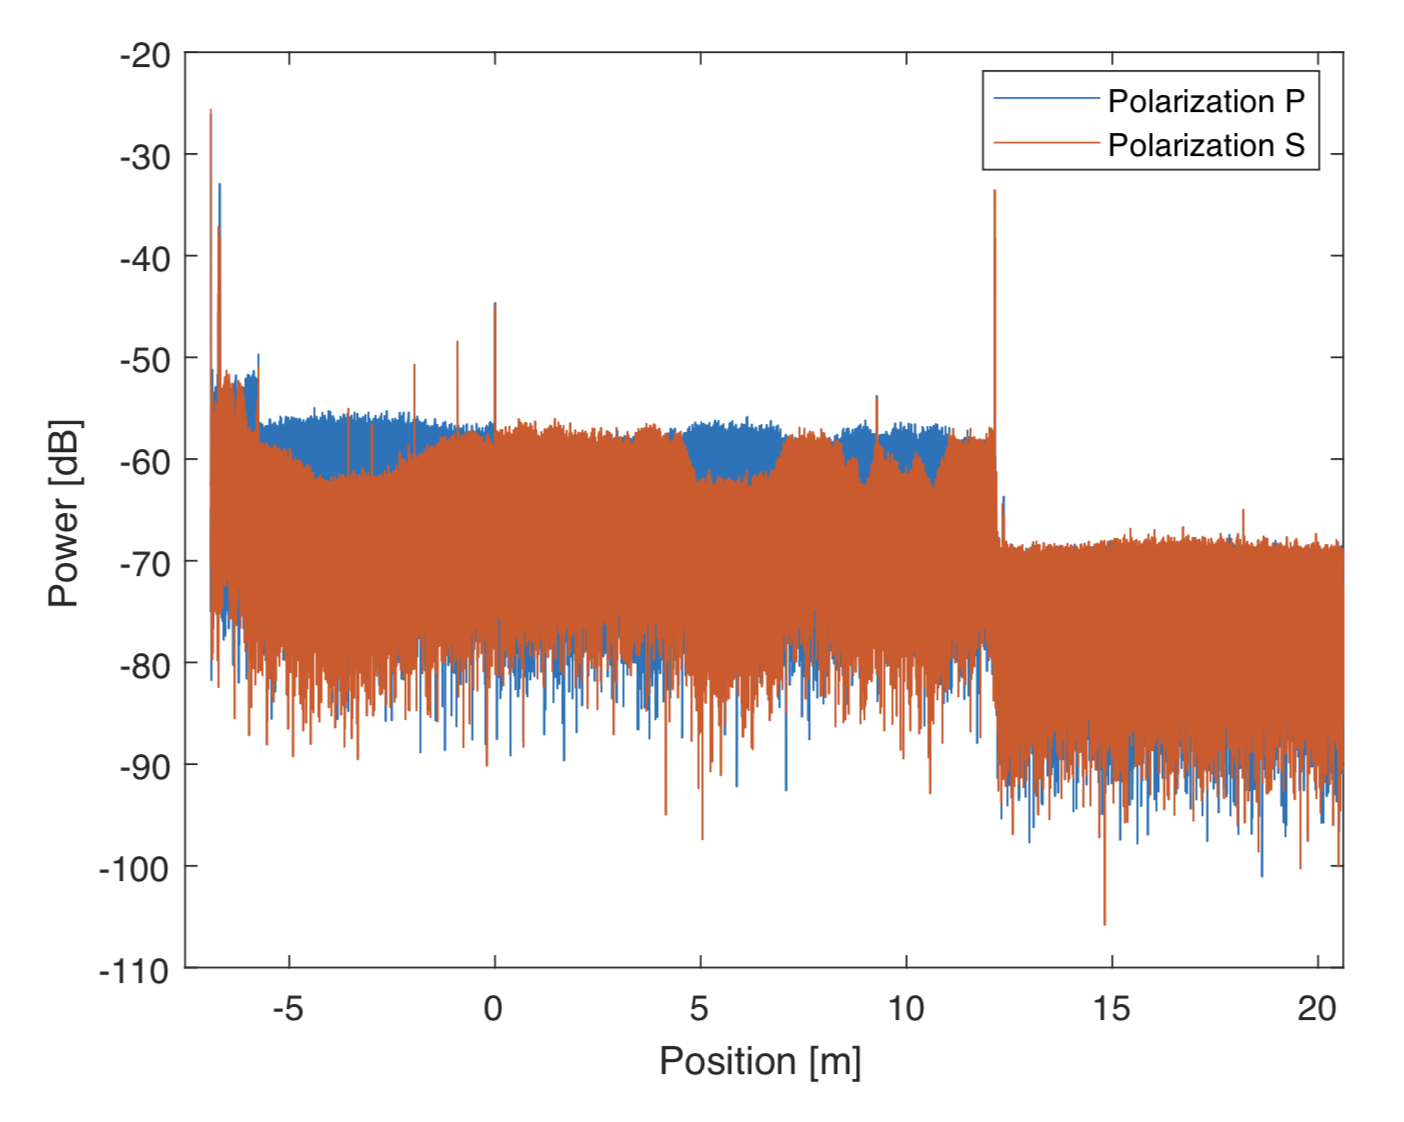
\includegraphics[height=10.5cm, width=10.5cm, keepaspectratio]{img/raw.png}
	\caption{Raw data}\label{fig:raw}
\end{figure}

The portion of the fiber of interest goes from 6,77 m (start of the sensor) to the final reflection peak at 12,1 m.

\lvlii{Numerical results}

A reference measure has been taken with no strain applied (fiber fingerprint): the sensor's final measure is obtained by correlating the latter with the measurement taken when the weight is applied.
The process described below has been performed for each weight applied.
As already mentioned, the received signal is the complex envelope of the electric field as a function of the position. Once the space coordinates are known, it is immediate to switch to the time domain, remembering that the optical distance includes also the backward backscattering signal (round trip): $z(t) = \frac{c_0 \cdot t_{TOT}}{2 n_{eff}}$

Given the reference measurement and the measurement with the weight applied, we want to find the spectral shift between the two: it is therefore necessary to work in the frequency domain.
To pass in the frequency domain maintaining a local information of the signal, it has been decided to perform the Discrete Fourier Transform (DFT) on a sufficiently small interval (window) instead of on the whole domain. The choice of the size of the window is a trade-off between ensuring local information, i.e., two points that are affected by a significantly different strain must belong to two different windows, and an adequate accuracy. We decided for a window size of 5 cm since it resulted as the best solution in terms of results after some numerical simulations.
The signal we have considered for our analysis is given by the sum of the amplitudes squared of the S and P spectra, in the selected window.
At this point, one can proceed to define the frequency shift between the signal with the applied weight and the reference signal. The spectral shift is given by the position of the cross-correlation peak (phase lag index) between the reference spectrum and the measured spectrum, properly converted in frequency.
If in a selected window there are \textit{w} samples spaced \textit{dt} seconds apart, the frequency resolution \textit{dF} of the spectrum is given by the opposite of the signal duration \textit{T}, with \textit{T}= \textit{w} \textit{dt}.


The cross-correlation between the two signals has been calculated, and in Fig. \ref{fig:xcross} is represented an example. We can then proceed with the detection of the peak.
\begin{figure}[H]
	\centering
	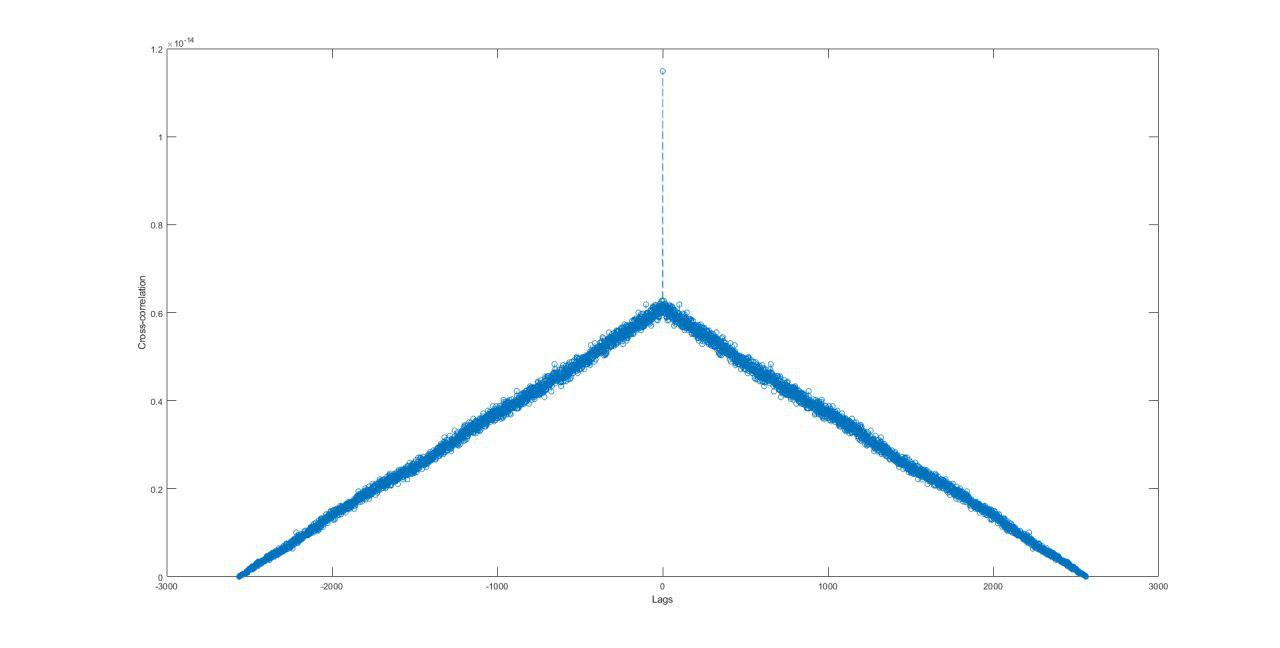
\includegraphics[height=10.5cm, width=10.5cm, keepaspectratio]{img/xcross.jpg}
	\caption{Cross-correlation}\label{fig:xcross}
\end{figure}
To make the analysis easier, it has been decided to subtract the mean value to each signal used to make the cross-correlation, as can be seen in Fig.\ref{fig:xcross-mean}
\begin{figure}[H]
	\centering
	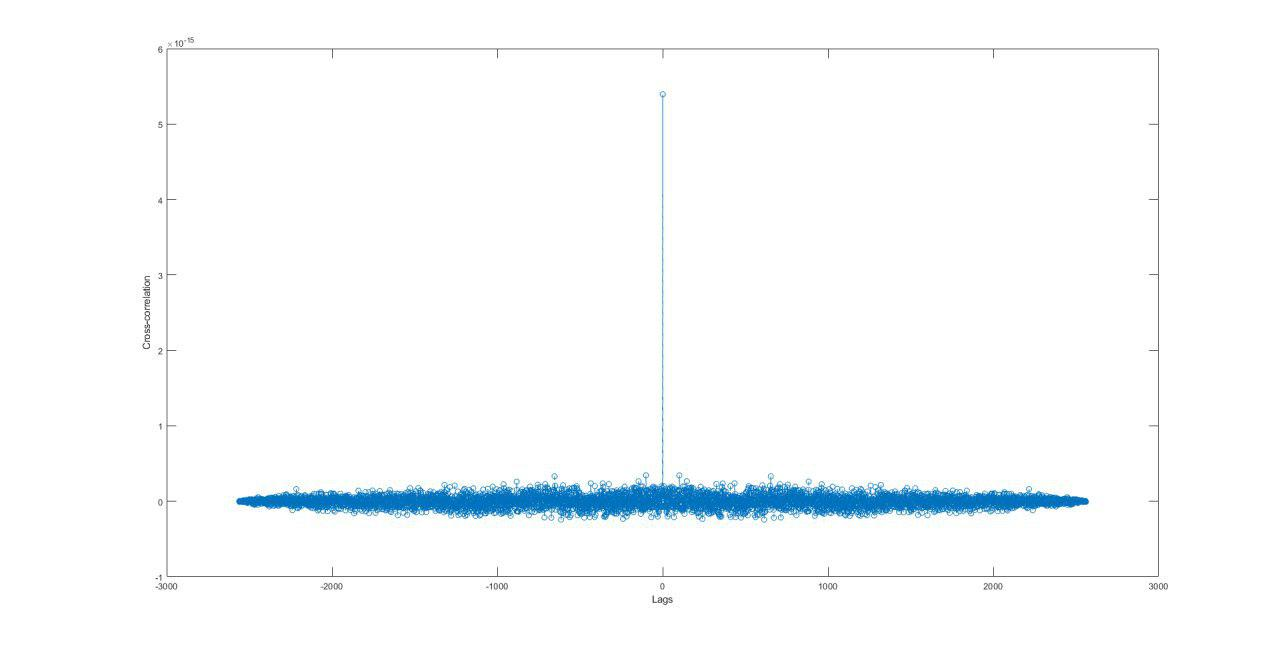
\includegraphics[height=10.5cm, width=10.5cm, keepaspectratio]{img/xcross-mean.jpg}
	\caption{Cross-correlation minus mean}\label{fig:xcross-mean}
\end{figure}
At this point, to find the maximum value, we apply a quadratic fitting using a parabolic approximation. Unfortunately, as can be noticed in Fig.\ref{fig:3points}, in the peak region we have only of 3 points, that are not sufficient to obtain a good estimate. In fact, we need at least 4 points of analysis that correspond to one point more than the degrees of freedom of the parabola.
\begin{figure}[H]
	\centering
	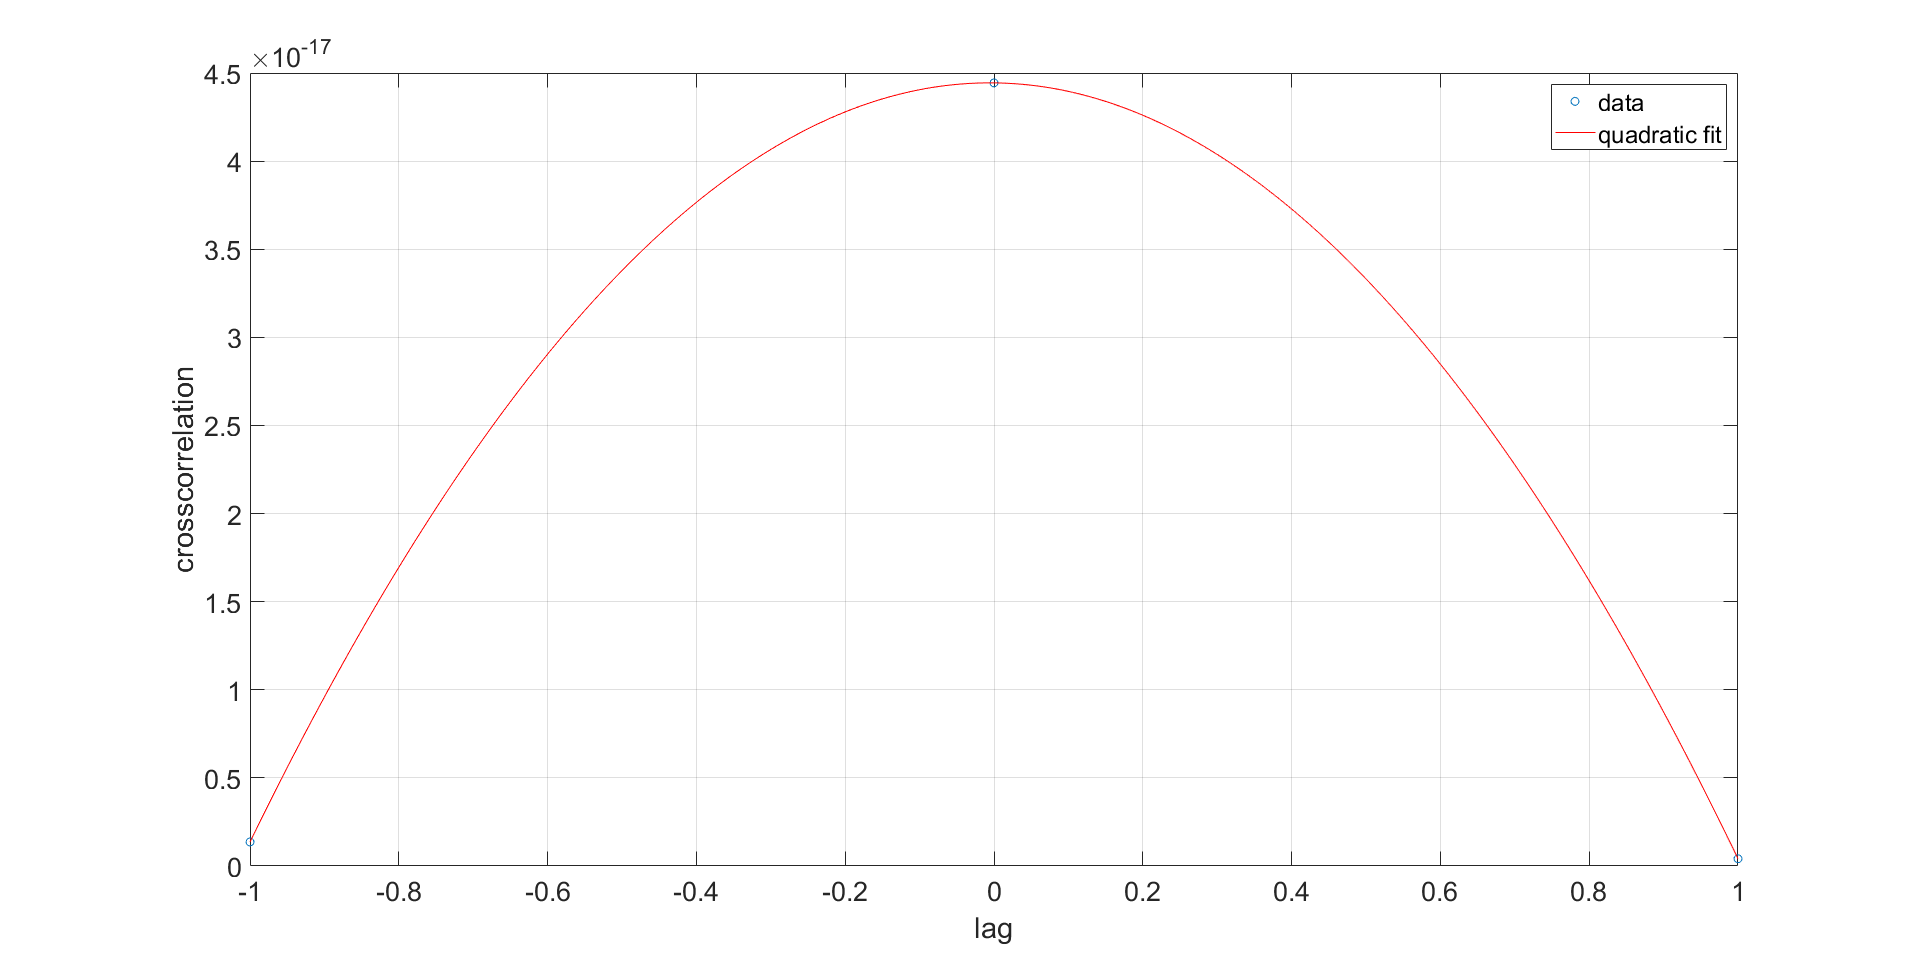
\includegraphics[height=10.5cm, width=10.5cm, keepaspectratio]{img/3points.png}
	\caption{Cross-correlation peak zoom}\label{fig:3points}
\end{figure}

For this reason, we have interpolated the DFTs by zero padding, fixed at 10. The spectral resolution does not varies. Data can hence be fitted with the quadratic interpolation, as represented in Fig. \ref{fig:10padding}.

\begin{figure}[H]
	\centering
	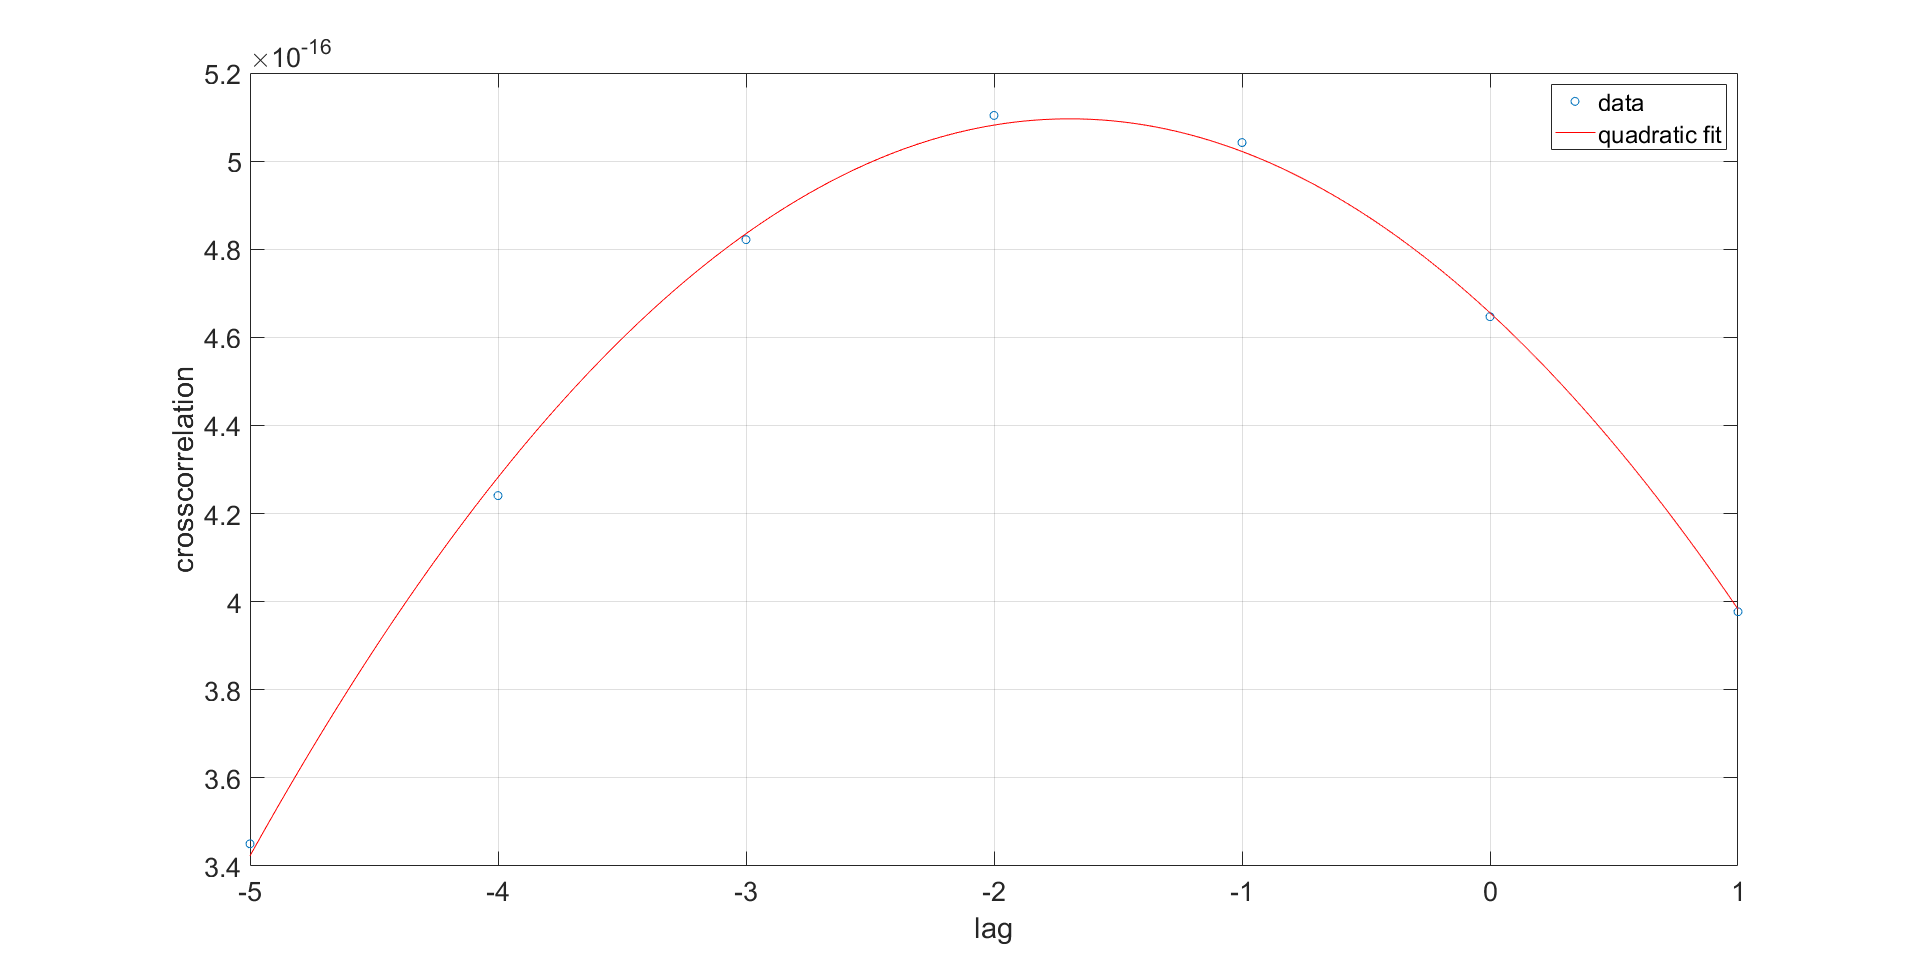
\includegraphics[height=10.5cm, width=10.5cm, keepaspectratio]{img/padding10.png}
	\caption{Cross-correlation with padding}\label{fig:10padding}
\end{figure}

The lag is then extracted and converted in a frequency shift, remembering to consider also the zero-padding.
The two windows (one for the reference and one for the strain measure) have been shifted together in order to have a spectral shift and hence a strain measure for each centimeter (window-step of 1 cm).

In this way, it has been possible to obtain the spectral shift $\delta$f (in GHz) as a function of the position along the fiber. As already mentioned, strain and spectral shift are related by:
\begin{center}
$ \delta f=k_{e}\delta \epsilon $
\end{center}
with $k_{e}$ = -0.15, and the strain measured in microstrain ($strain*10^{-6}$) . The results are firstly shown for a particular weight applied (782 g, the maximum weight), in order to highlight the different features applied during the processing of the data. In the following figures: in Fig.\ref{fig:nofit} and in Fig. \ref{fig:final} is represented the microstrains without the fitting (left) compared with the processing final result (right).

\begin{figure}[H]
    \minipage{0.50\textwidth}
    \centering
    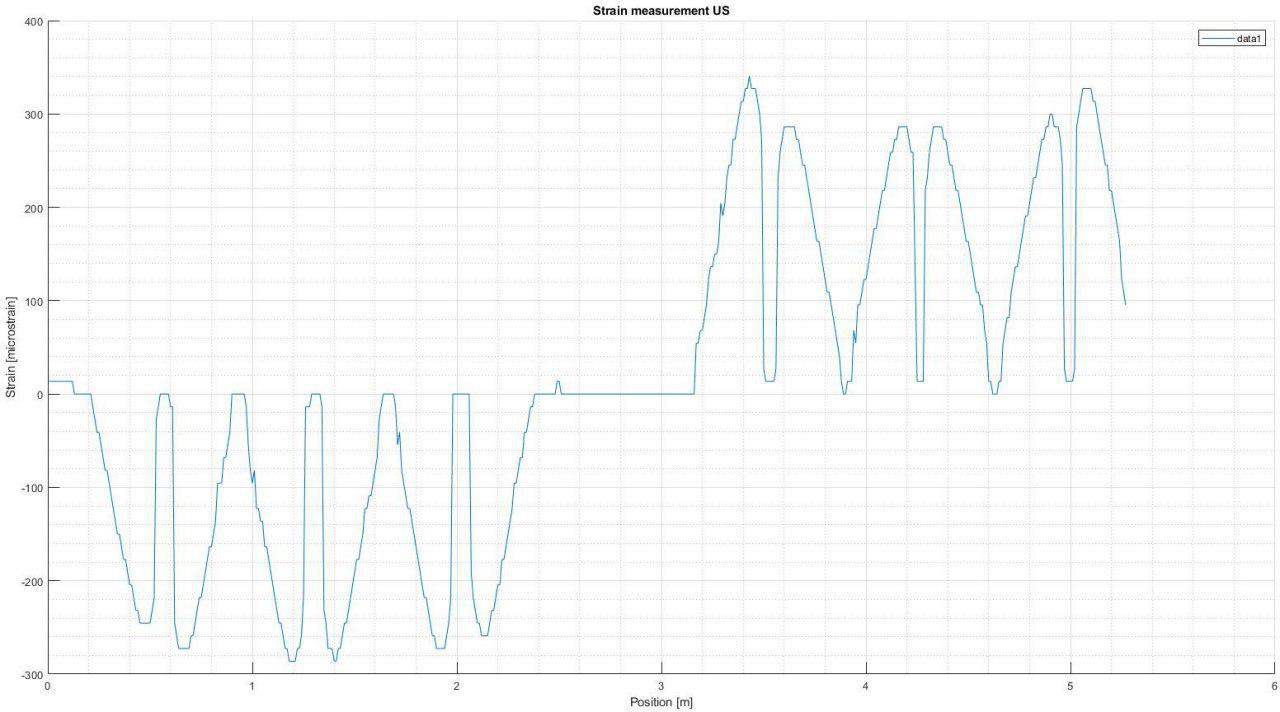
\includegraphics[scale=0.25]{img/nofit.jpg}
    \caption{Raw microstrain.}
    \label{fig:nofit}
    \endminipage\hfill
    \minipage{0.50\textwidth}
    \centering
    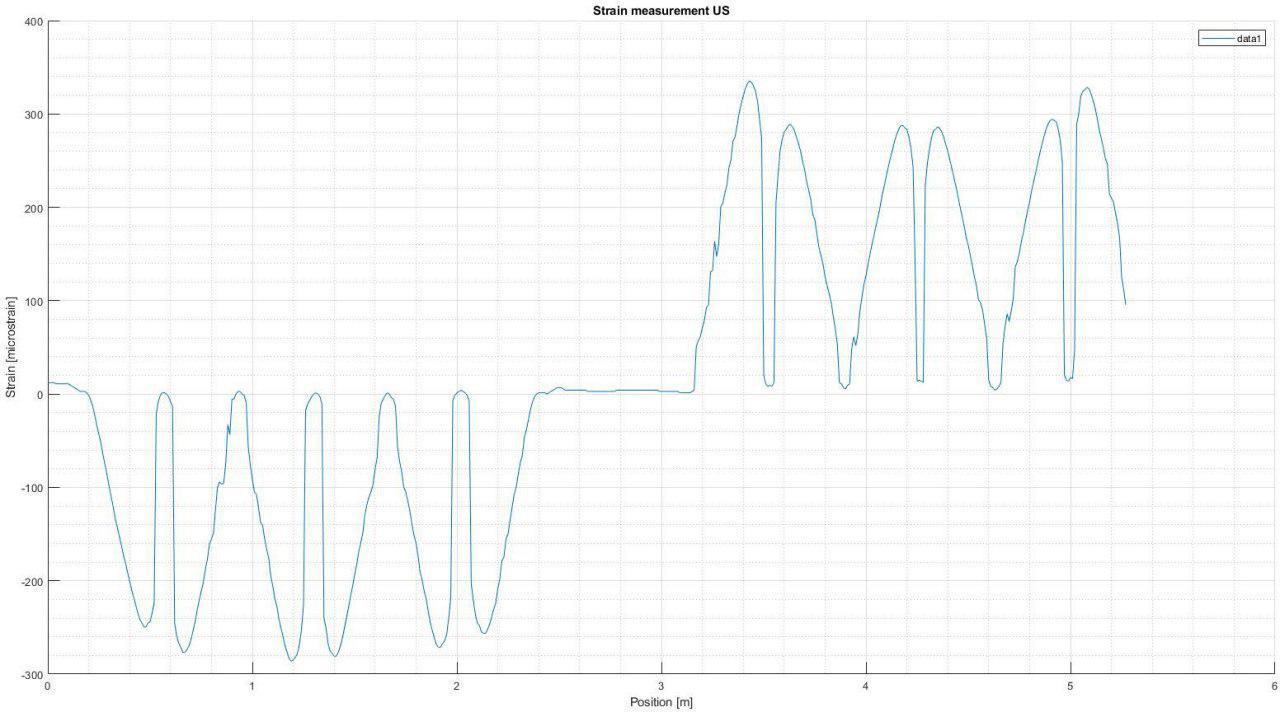
\includegraphics[scale=0.25]{img/final.jpg}
    \caption{Final microstrain.}
    \label{fig:final}
    \endminipage
\end{figure}

The processed results (Fig.8) are smoother than the raw ones. The final results for all the weights applied are shown in Fig. \ref{fig:strain}

\begin{figure}[H]
	\centering
	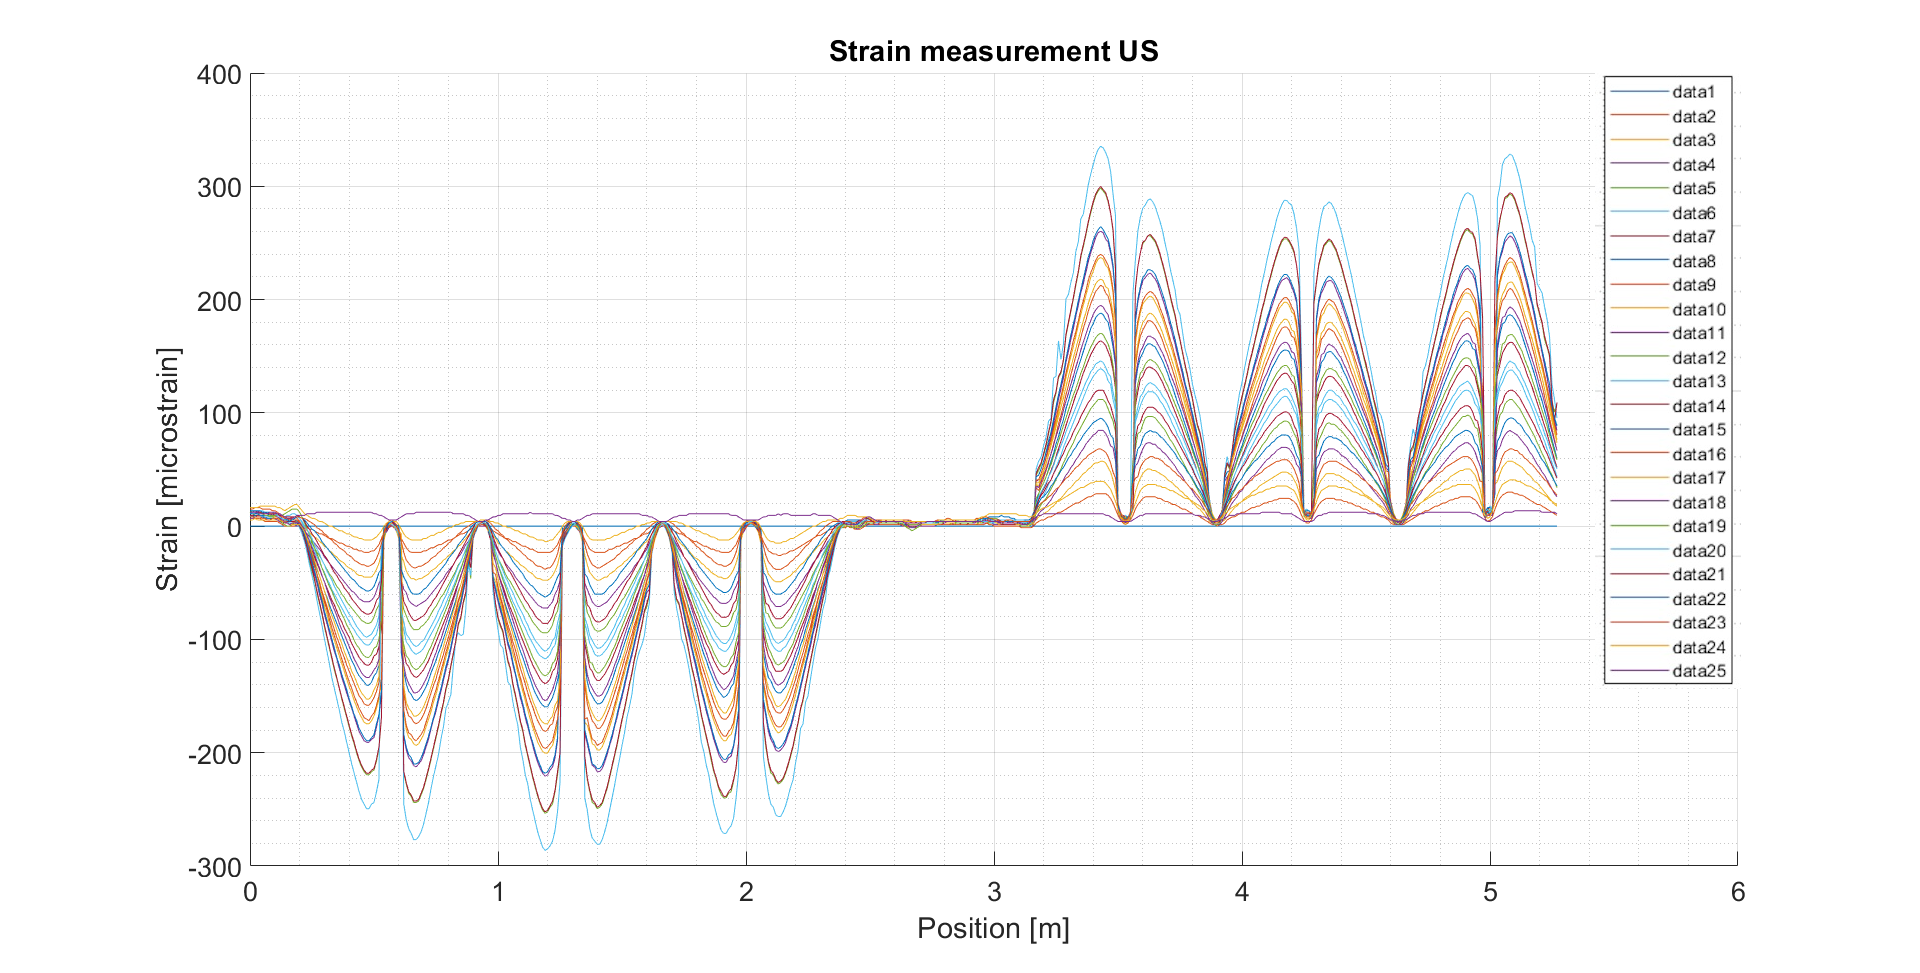
\includegraphics[height=10.5cm, width=10.5cm, keepaspectratio]{img/nostro.png}
	\caption{Resulting plot for each weight applied}\label{fig:strain}
\end{figure}

It is clear that the signals obtained comply with the setup scheme: the first portion of the fiber sensor has a negative value of strain and corresponds to the compression of the fiber under the table, while the final part is positive and corresponds to the lengthening of the fiber upon the board. The values of strain deduced from the graphs correspond to the values taken during the laboratory experience and reported in the third and fourth column of Table 1.



\lvli{Discussion and Conclusions}

To verify the goodness of our measurements, we have plotted in Fig. \ref{fig:sensitivity} the microstrains as a function of the applied weight, in a specific position in the fiber.  The position chosen was a point of maximum strain to obtain the highest possible sensitivity of the device, estimated as the slope of a linear fitting. In red, the measurements obtained applying increasing weight (forward direction), while in blue the ones in the opposite direction. The values of sensitivity obtained are $S_f = 0.4229$ $\mu \varepsilon / g$ for the forward direction, and $S_b = 0.4074$ $\mu \varepsilon / g$ for the backward direction.

\begin{figure}[H]
	\centering
	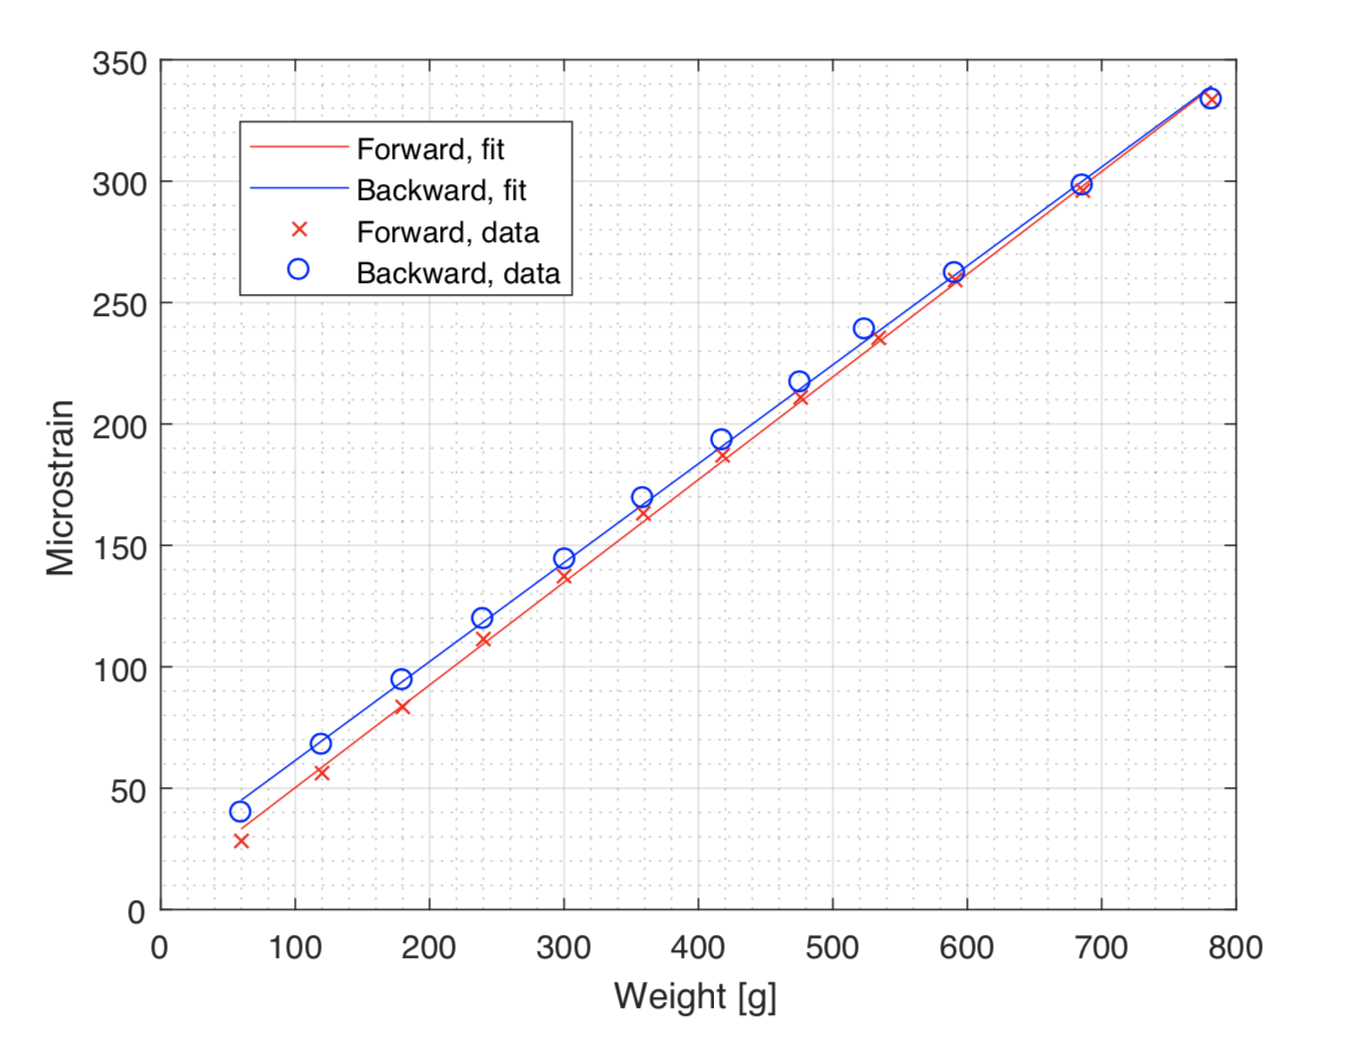
\includegraphics[height=10.5cm, width=10.5cm, keepaspectratio]{img/sensitivity.png}
	\caption{Microstrain versus weight applied}\label{fig:sensitivity}
\end{figure}

It can be noticed that the forward and backward curves are not overlapping: supposedly, this is due to the change in temperature occurred during the experiment that is more evident comparing the first and the final measurements.


Our final results have been compared with the ones of the device, that are plotted in Fig. \ref{fig:OFDR}.

\begin{figure}[H]
	\centering
	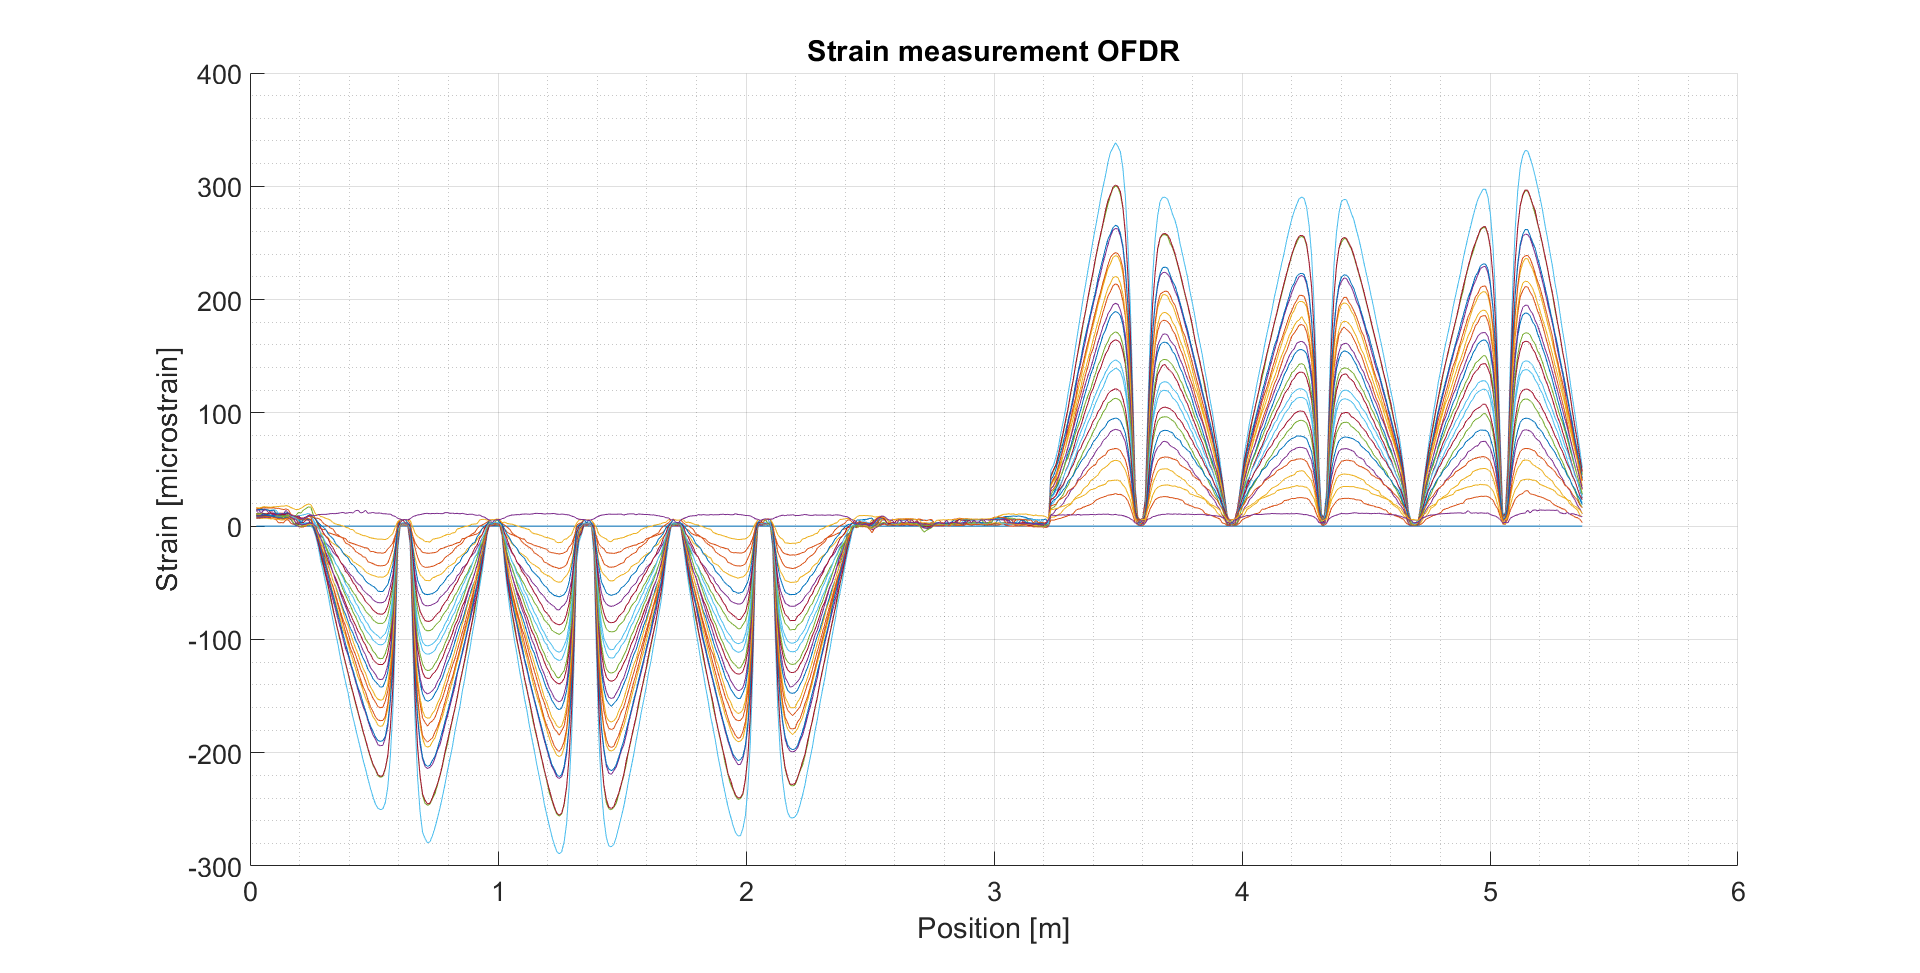
\includegraphics[height=10.5cm, width=10.5cm, keepaspectratio]{img/OFDR.png}
	\caption{OFDR data for each weight applied}\label{fig:OFDR}
\end{figure}

The superposition of the two results are represented in Fig. \ref{fig:sovrapposizione}, considering that the OBR processing of the data is not known, the results are substantial.

\begin{figure}[H]
	\centering
	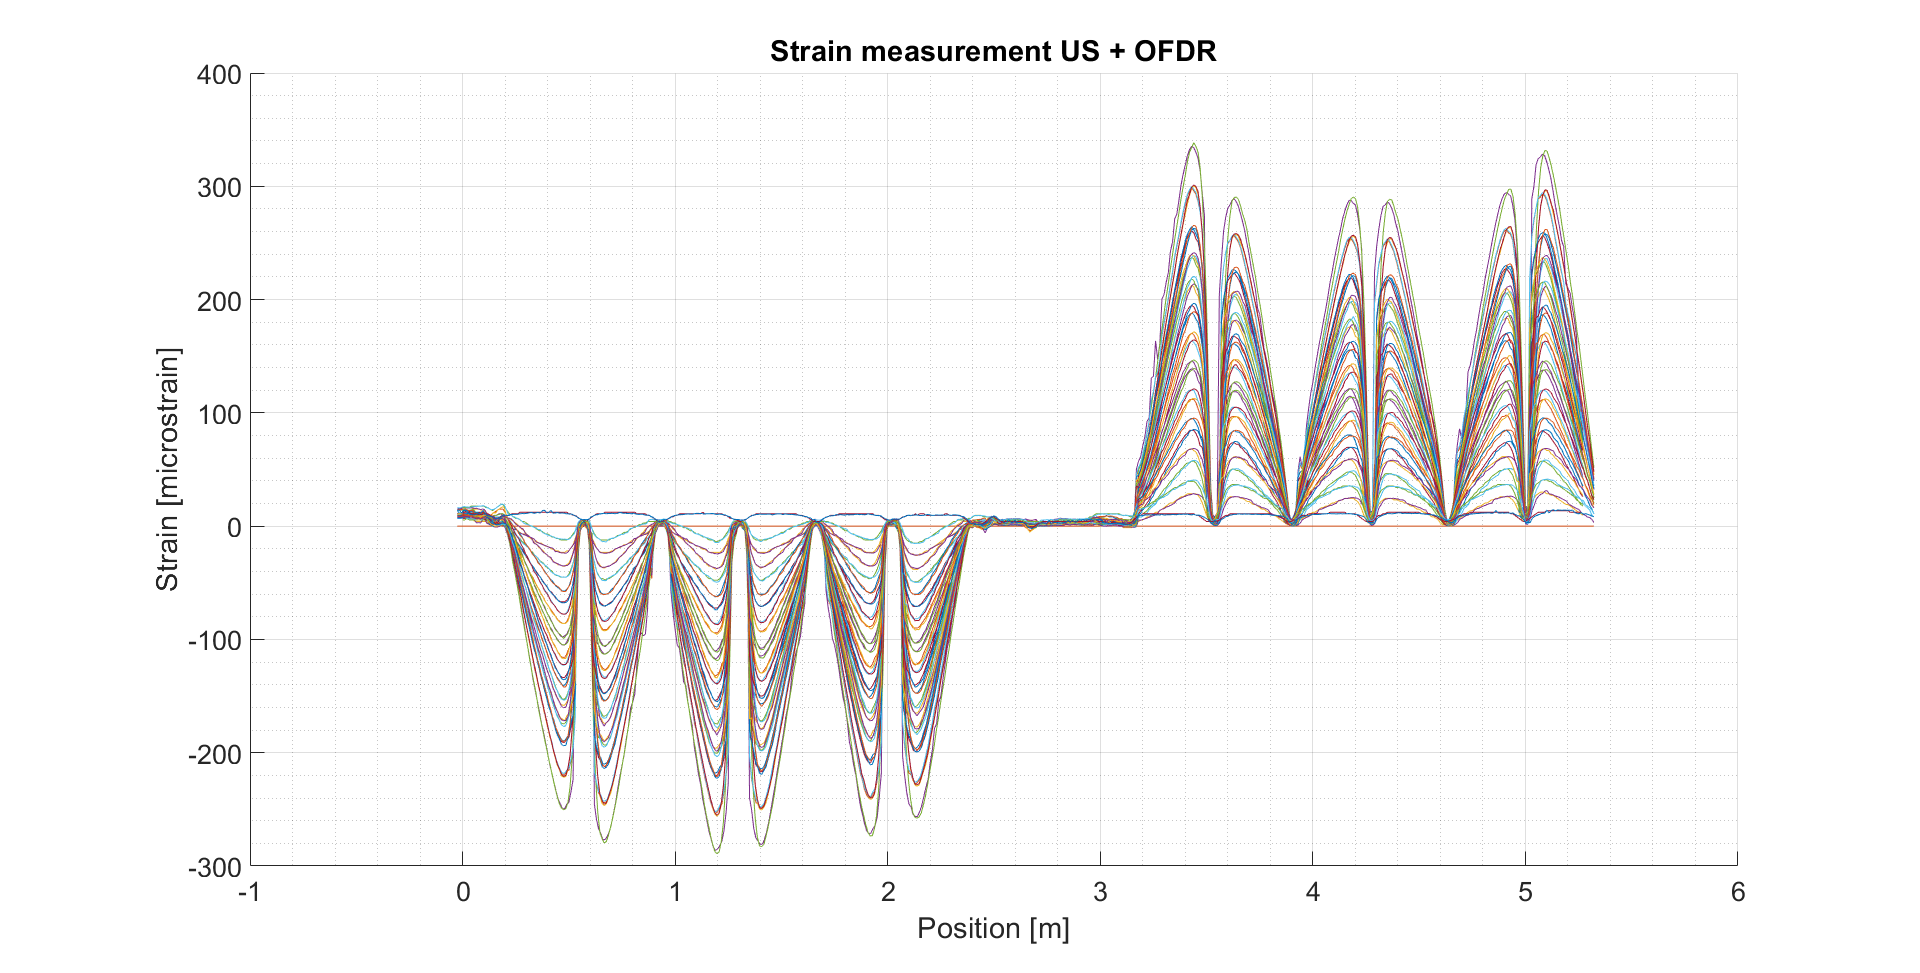
\includegraphics[height=10.5cm, width=10.5cm, keepaspectratio]{img/sovrapposizione.png}
	\caption{Comparison between ours and OBR's processed data }\label{fig:sovrapposizione}
\end{figure}

In conclusion, this experiment confirms that it is possible to use a distributed fiber sensor coupled mechanically with the object of interest to perform a measure of strain. Since the results we have obtained autonomously are substantial with the ones of the OBR commercial device, we can conclude that the backscattering signal analysis is a good tool to perform strain measures.




\lvli{Appendix}
One way to understand the goodness of our analysis was to compare it with the one carried out automatically by the OBR, this analysis is qualitative because we do not know with certainty the calculations performed by the OBR. The files that supplies us in output contain, in particular, two columns that provide us with information on the frequency shift with respect to the position. To have an indicative estimate of how much it differs from ours it was decided to carry out a statistical analysis on the difference between the two graphs:
$$g(x) = f_2(x) - f_1(x)$$
To make the point-to-point difference we needed the two graphs to have the same sampling, so it was decided to perform a spline interpolation on both and resample the two signals with 1000 points, the resulting signal is shown in Fig. \ref{fig:difference}.
%figura%
\begin{figure}[H]
	\centering
	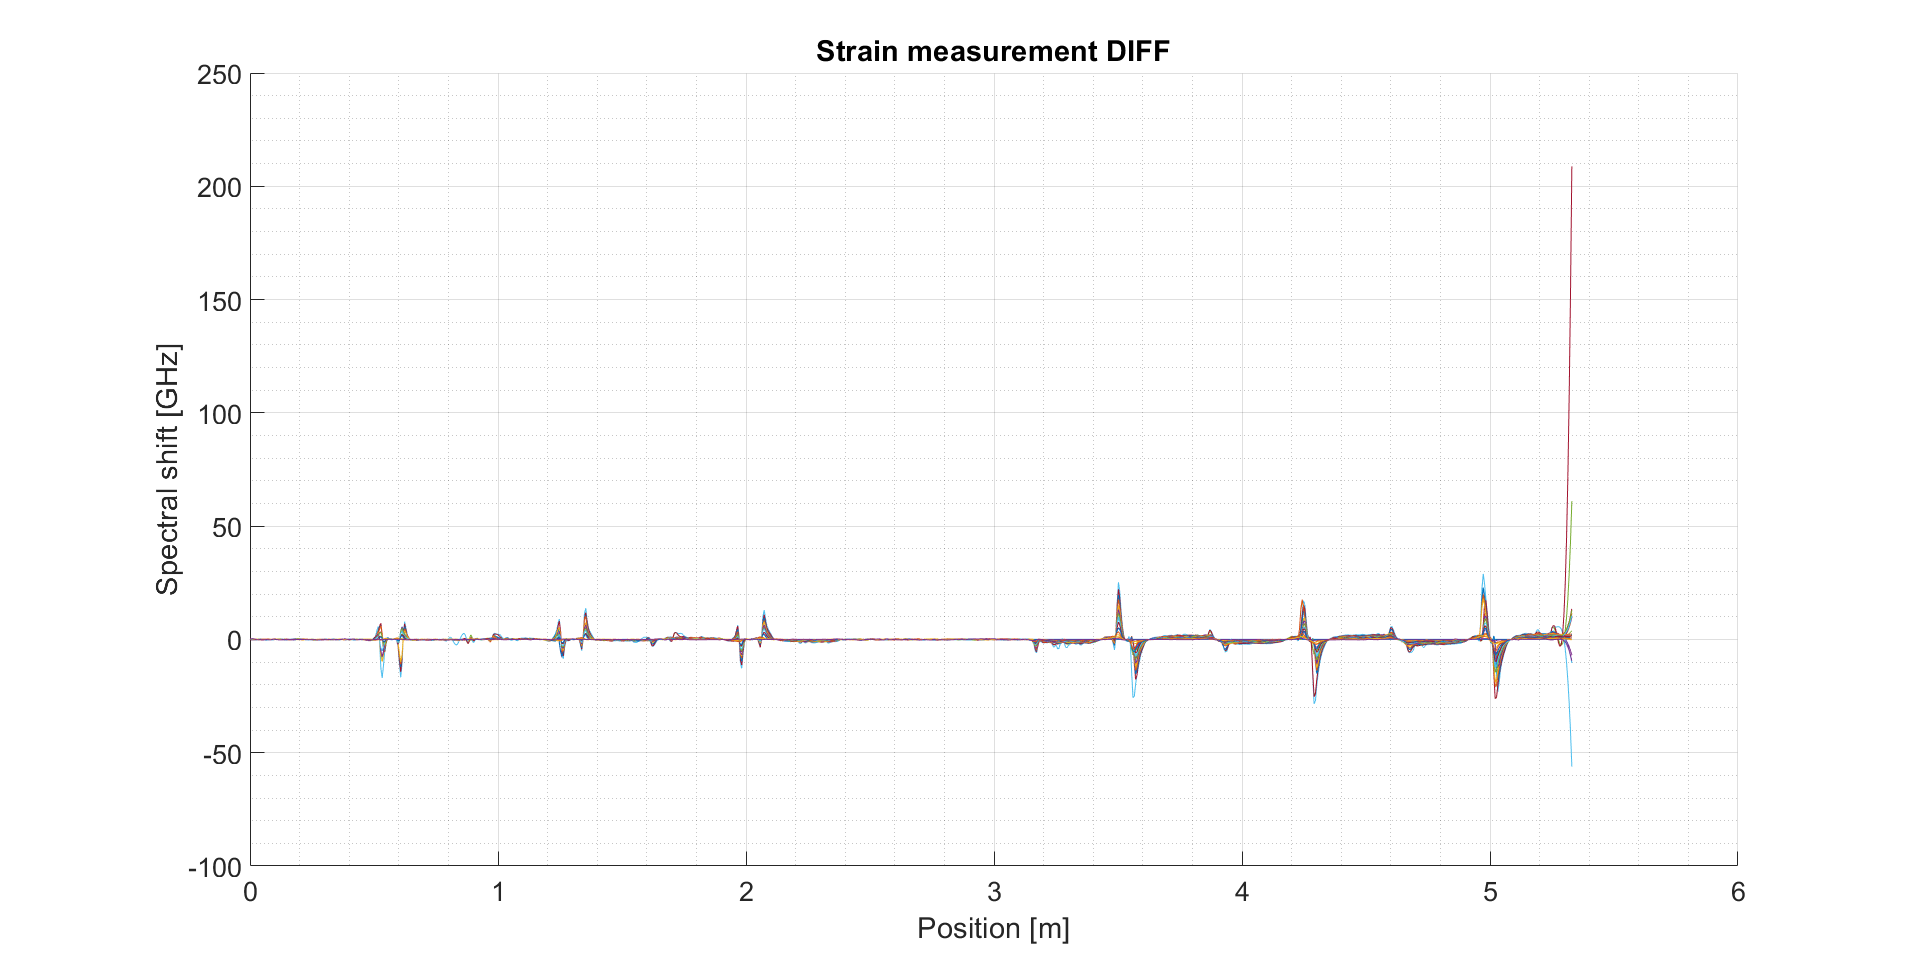
\includegraphics[scale=0.3]{img/diff.png}
	\caption{$g(x)$ for each signals.}\label{fig:difference}
\end{figure}
The last part of the signal (about 7 points) has some peaks introduced by the edge effects of the fitting using splines and therefore should not be taken into consideration therefore the calculations were made without taking it into consideration.
For each measurement the variance of the difference signal was calculated and the normalized mean of the difference signal compared to the average of our signal; the given data have been reported in the table Tab. \ref{table:difference}. Look at the values of the average we can derive a possible systematic error between the two references, in our case all the values are low and are below 10\% with the sole exception of the signal 14. With regard to the variance we can deduce an increase of noise of our signal compared to that of the OBR with the increase of weight, the difference is not easily attributable to a specific cause because we do not know the complete post processing of the instrument, we can imagine depends on any calculations and or parameters performed differently .

\begin{table}[h]
\centering
 \begin{tabular}{c|c|c}
    measure & normalized mean & variance \\
    \hline
		1 &    0     &  0    \\
		2 &    0.02  &  0.07 \\
		3 &    0.04  &  0.25 \\
		4 &    0.05  &  0.60 \\
		5 &    0.07  &  1.19 \\
		6 &    0.05  &  1.76 \\
		7 &    0.03  &  2.50 \\
		8 &    0.02  &  3.03 \\
		9 &    0.07  &  4.75 \\
		10 &   0.01  &  7.23 \\
		11 &   0.01  &  7.53 \\
		12 &   0.08  & 11.35 \\
		13 &   0.07  & 16.42 \\
		% \hline
		14 &   0.10  & 11.52 \\
		15 &   0.01  &  7.54 \\
		16 &   0.00  &  7.50 \\
		17 &   0.03  &  5.53 \\
		18 &   0.01  &  3.15 \\
		19 &   0.02  &  2.64 \\
		20 &   0.02  &  1.89 \\
		21 &   0.01  &  1.17 \\
		22 &   0.01  &  0.71 \\
		23 &  -0.00  &  0.36 \\
		24 &  -0.01  &  0.10 \\
		25 &   0.03  &  0.01 \\
 \end{tabular}
\caption{Statistical comparison between our data and the OBR data.}
 \label{table:difference}
\end{table}
